% Load the base class
\documentclass[minted, draw]{../tex/hebdomon}
\usepackage{svg}
\begin{document}

\title{Blood Cells Detection and Classification using Deep Learning and Machine Learning}
\author{v0.1}
\StudentName{Achille Cannavale}
\date{dtm@mci4me.at}

\publishers{
  \begin{tabular}[!b]{rl}
  \textbf{Student Name} & Achille Cannavale \\[3pt]
  \textbf{Student Number} & xxxxx \\[3pt]
  \textbf{Module Name} & xxxxx
  \end{tabular}\\[20pt]
  }

\begin{titlepage}
    \centering
	
\includegraphics[width=4cm]{figures/logo.png}\par\vspace{1cm}

    %\vspace*{2cm}

    {\scshape\LARGE Università degli Studi di Cassino e del Lazio Meridionale\par}
    \vspace{1cm}
    {\Large Corso di Laurea Magistrale in Ingegneria Informatica \par}

    \vspace{2cm}
    {\Huge\bfseries Blood Cells Detection and Classification using Deep Learning and Machine Learning\par}
    \vspace{1cm}
    {\large Versione 0.1}

    \vfill

    \begin{flushleft}
    \textbf{Cannavale Achille} \\
    \textbf{Colacicco Nunziamaria} \\
    \textbf{La Torre Noemi} \\
    \end{flushleft}

    \vspace{1.5cm}

    {\large \today\par}
\end{titlepage}

\dominitoc
\tableofcontents
\newpage

\Chapter{}
\Section{Introduzione}

La malaria è una delle principali malattie infettive a livello globale, con un impatto significativo sulla salute pubblica, in particolare nei paesi tropicali e subtropicali. Tra i diversi parassiti responsabili di questa patologia, il \hlight{Plasmodium vivax} rappresenta una delle specie più diffuse. La diagnosi precoce e accurata è fondamentale per un trattamento tempestivo ed efficace, e l’analisi microscopica degli strisci ematici rimane uno degli strumenti diagnostici più affidabili.
In questo progetto, viene affrontato il problema della rilevazione e classificazione automatica delle cellule del sangue infettate da P. vivax, attraverso tecniche di machine e deep learning.
Utilizzando il dataset \hlight{P. vivax malaria infected human blood smears}, che contiene oltre \textbf{1.300} immagini microscopiche annotate con più di \textbf{86.000} cellule identificate e classificate, si propone una pipeline [FOTO] che combina \textbf{Deep Learning} e \textbf{Machine Learning} per:

\begin{itemize}
	\item individuare automaticamente le regioni di interesse (ROI) contenenti cellule
	\item estrarre le feature significative dalle ROI
	\item classificare ogni cellula in una delle categorie predefinite, tra cui cellule sane (red blood cell e leukocyte) e diversi stadi del parassita infetto (trophozoite, ring, gametocyte, schizont)
\end{itemize}

\begin{warning}
	L’analisi di questo lavoro ha evidenziato una marcata sbilanciatura del dataset, aspetto che ha richiesto un’attenta progettazione delle strategie di addestramento.
\end{warning}
%
\begin{figure}[ht]
	\centering
	\includesvg[width=\linewidth]{figures/pipeline_general.svg}
	\caption{Pipeline Generale del nostro progetto, suddivisa in una fase di Deep Learning per per la rilevazione delle ROI e l'estrazione delle features e una fase di Machine Learning per la classificazione delle cellule.}
\end{figure}
%

\Section{Strumenti utilizzati}

Per lo sviluppo del progetto sono stati adottati diversi strumenti software, suddivisi in base alle funzionalità specifiche per il \textit{deep learning}, il \textit{machine learning} e l’analisi dei dati. La scelta di ciascuno di essi è stata guidata da criteri di efficienza, semplicità d’uso e ampia diffusione nella comunità scientifica.

\begin{itemize}
    \item \textbf{Deep Learning:} \textit{PyTorch} \\
    Utilizzato per la progettazione, l’addestramento e la valutazione dei modelli di deep learning. PyTorch si distingue per la sua flessibilità e l’approccio dinamico alla costruzione delle reti neurali, risultando particolarmente adatto per attività di ricerca e prototipazione rapida.

    \item \textbf{Machine Learning:} \textit{Scikit-learn} \\
    Impiegato per l’implementazione di algoritmi di machine learning tradizionali, grazie alla sua vasta collezione di modelli predefiniti e strumenti per la valutazione delle prestazioni.

    \item \textbf{Strumenti Ausiliari:}
    \begin{itemize}
        \item \textit{NumPy} e \textit{Pandas}: utilizzati per la manipolazione, la pulizia e l’analisi dei dati, fondamentali nella fase di preprocessing e gestione dei dataset.
        \item \textit{Matplotlib}: utilizzata per la visualizzazione grafica dei risultati, utile per l’analisi esplorativa e la presentazione delle performance dei modelli.
    \end{itemize}
\end{itemize}

\Section{Composizione Dataset}

Il dataset utilizzato per questo progetto è composto da \textbf{1.328 immagini} contenenti in totale \textbf{86.035 oggetti annotati}. Ogni oggetto rappresenta una singola cellula o elemento biologico rilevato nelle immagini microscopiche, ed è associato a una delle seguenti \textbf{sette classi}:

\begin{itemize}
    \item \texttt{red blood cell} (83.034)
    \item \texttt{trophozoite} (1.584)
    \item \texttt{ring} (522)
    \item \texttt{difficult} (446)
    \item \texttt{schizont} (190)
    \item \texttt{gametocyte} (156)
    \item \texttt{leukocyte} (103)
\end{itemize}

Come si può osservare dalla distribuzione, il dataset presenta un \textbf{forte sbilanciamento tra le classi}, con la stragrande maggioranza degli oggetti appartenenti alla categoria \texttt{red blood cell}, che rappresenta da sola circa il \textbf{96{,}5\%} del totale.

Questo sbilanciamento costituisce una \textbf{sfida rilevante per i modelli di classificazione}, in quanto tende a favorire la previsione della classe dominante a discapito delle classi minoritarie, che possono essere trascurate o predette con bassa accuratezza.

%Per affrontare questo problema, durante lo sviluppo sono state considerate diverse strategie, tra cui:
%\begin{itemize}
%    \item il bilanciamento del dataset,
%    \item l’uso di tecniche di \textit{data augmentation},
%    \item l’assegnazione di pesi differenti alle classi durante l’addestramento,
%    \item e l’adozione di metriche di valutazione più robuste rispetto alla sola accuratezza, come \textit{precision}, \textit{recall} e \textit{F1-score}.
%\end{itemize}


\Section{Title Formatting1}
ciao noemi
To begin a new content, always start the content with a chapter heading. To
insert the chapter with an additional \lstinline[columns=fixed]{minitoc}
use \lstinline[columns=fixed]{\Chapter}, which produces an heading as
you see at the beginning of this page, to have a heading without
a \lstinline[columns=fixed]{minitoc} use the standard
\lstinline[columns=fixed]{\chapter}.

The document relies on the user to use the \hlight{correct} title commands to
keep the formatting consistent. The commands that starting with a
capital letter are the overloaded commands of the standard ones.
The following are the current ones:
%
\begin{code}{python}
\Chapter{...}
\Section{...}
\Subsection{...}
\Subsubsection{...}
\end{code}
%
\begin{warning}
	Unless there is a specific reason, it is suggested to use the aforementioned
	commands. However, original LaTeX command should work as well if you want to use.
\end{warning}

\Subsection{Page Geometry}

The page geometry is set to the following settings. This is done using the
standard package \pcode{\usepackage{geometry}} which is defined in the
\pcode{Hebdomon.cls}.
%
\begin{itemize}[leftmargin=!,labelindent=-29.2pt]
	\item[\textbf{top}] 2.5cm,
	\item[\textbf{right}] 2.0cm,
	\item[\textbf{bottom}] 2.5cm,
	\item[\textbf{left}] 3.0cm.
\end{itemize}
%
\Section{Image Positioning}
%
The image positioning could be done with the following code snippet:
%
\begin{code}{latex}
\begin{figure}[ht]
  \centering
  \includegraphics[options]{figures/path.pdf}
  \caption{\label{fig:label} }
\end{figure}
\end{code}
%
Here there are a few options worth mentioning:
%
\begin{hgitemize}
	\item[\pcode{figures/path}] The place where the image is kept. If the
	image is in the same folder where the main.tex file resides, it is as
	simple as writing the files name. If the file is in a folder called
	image, just write \pcode{image/innsbruck.jpg}. Finally if the image is
	in a higher directory (i.e., image is in folderA/innsbruck.jpg and the
	main tex is in folderA/document/main.tex then the path becomes \pcode{../innsbruck.jpg}
	\item[\pcode{\caption{..}}] Where you write the caption of the image.
	For consistency make sure every image has a caption as if the image does not
	need a caption, maybe it not be present to begin with.
	\item[\pcode{label{}}] This is an identifier for you to use when you need
	to cite this Figure in a place somewhere. For example if you were to have
	and image with the following:
\end{hgitemize}
%
\begin{code}{latex}
\begin{figure}[ht]
  \centering
  \includegraphics[width=\textwidth]{figures/path.pdf}
  \caption{A photo I found on the web.}\label{fig:innsbruck}
\end{figure}
\end{code}
%
\begin{hgitemize}
	\item[] Now this image is referenced as \pcode{fig:innsbruck}, which
	means if we write the following:
\end{hgitemize}
%
\begin{code}{text}
To see the image, have a look at Figure \ref{fig:innsbruck}
\end{code}
%
This line of command will be presented as
%
\begin{excerpt}
	To see the image, have a look at Figure 1.1.
\end{excerpt}
%
Finally you can see the image here as well.
%
\begin{figure}[ht]
	\centering
	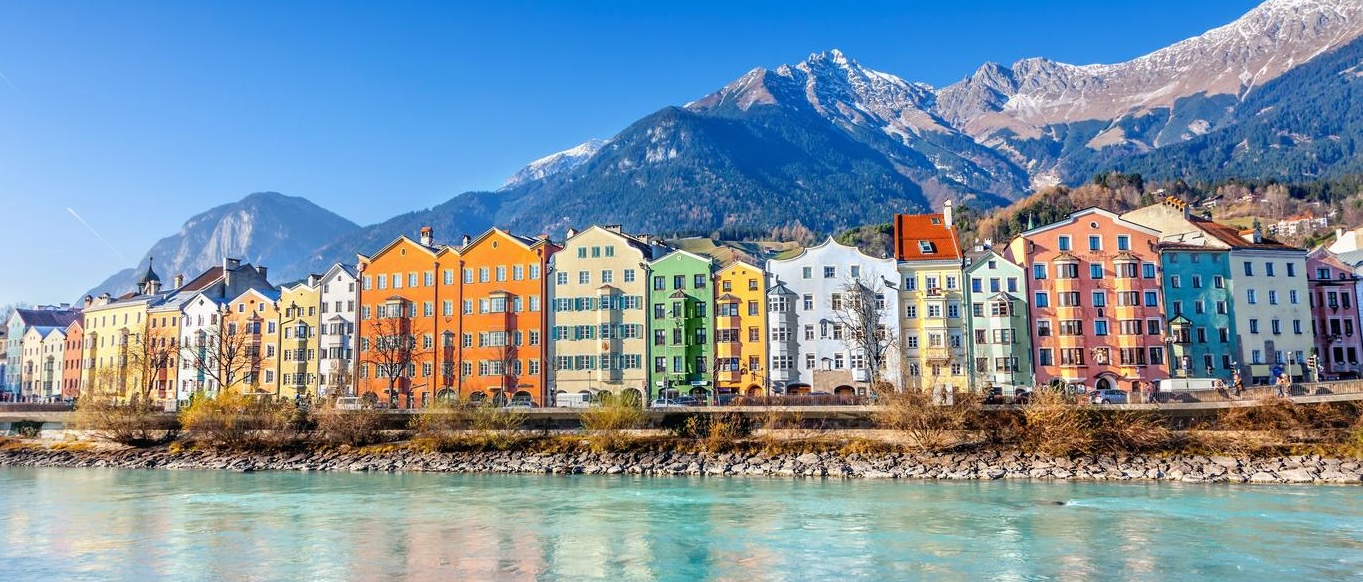
\includegraphics[width=\linewidth]{figures/innsbruck.jpg}
	\caption{The famous Innsbruck houses near the river Inn. This image is
		placed with a width value of \pcode{width=\linewidth}. This is also
		a good opportunity to showcase the hanging behaviour of the figure
		caption.}
\end{figure}
%
\Section{Defined Environments}
%
\begin{hgitemize}
	\item[\pcode{excerpt}] The template relies on the excellent \lstinline[columns=fixed]{tcolorbox}
	package for formatting the boxes within the document and for that end different styles were created.
	\item[] Sometimes one needs to quote either a proverb or to create drama, for this use
	the \lstinline[columns=fixed]{excerpt} environment with the following notation and effect.
\end{hgitemize}
%
\begin{code}{latex}
\begin{excerpt}
  To be, or not to be...
\end{excerpt}
\end{code}
%
\begin{hgitemize}
	\item[] Compiling this code snippet would show as in the document
\end{hgitemize}
%
\begin{excerpt}
	To be, or not to be...
\end{excerpt}
%
\begin{itemize}[leftmargin=!,labelindent=-29.2pt]
	\item[\pcode{code}] During the preparation of your document, it is useful to showcase
	      some code either in the shape of all the document or a snippet of it.
	      There are two (\hlight{2}) ways of doing this where the first one will be discussed here.
	\item[] For example to print out a hello world in python, please use the following environment
\end{itemize}
%
\begin{verbatim}
\begin{code}{python}
print("Hello, World!")
\end{code}
\end{verbatim}
%
Producing the following:
%
\begin{code}{python}
print("Hello, World!")
\end{code}
%
The class also come with some predefined environments to modify the behaviour/aesthetics of the document.
%
Highlighting text is \hlight{very easy}, here is an example on how to write one.

\begin{code}{latex}
Highlighting text is \hlight{very easy}, here is an example:
\end{code}

\begin{itemize}[leftmargin=!,labelindent=-29.2pt]
	\item[\pcode{example}] Sometimes you need to showcase an example or
	      need to highlight a certain idea.
	      For these things the environment Example could be useful.
	\item[] For example to show as simple example or give a slight attention to a topic you can do the following.
\end{itemize}

\begin{example}
	This is an example. This could be anything which you would like to have a certain amount of
	attention but not too much as to distract from the flow of the document.
\end{example}

\begin{itemize}[leftmargin=!,labelindent=-29.2pt]
	\item[\pcode{highlight}] Or sometimes you need to give a clear break to the flow of the
	      document and ask the reader to look at your banner. For that use highlight.
\end{itemize}

\begin{highlight}
	Hey! Pay attention as this is a highlight box.
\end{highlight}

\Subsection{Writing Equations}
%
One of the strong suits of LaTeX compared to other editors and programs is
it simplicity and ease of use methods of writing equations. Consider the
following equation:
%
\begin{equation*}
	f(x) = x^2 + 2x + 1
\end{equation*}
%
In code form this would be written as:
%
\begin{code}{latex}
	\begin{equation*}
		f(x) = x^2 + 2x + 1
	\end{equation*}
\end{code}
%
All equations that has their newline and centre staged are mostly written
in an environment where it has a \pcode{begin} and an \pcode{end}. You may
have noticed the asterisks sign just after the equation. This implies the
environment is \hlight{not numbered}, meaning you won't be able to
reference it. This is used to limit the numbering of equations to just the
essential parts in the document and not reach 3 digits by the time you are
in page 8. For a numbered equation like the following
%
\begin{equation}
	f(x) = x^2 + 2x + 1
\end{equation}
%
You only need to do:
%
\begin{code}{latex}
	\begin{equation}\label{eq:quad}
		f(x) = x^2 + 2x + 1
	\end{equation}
\end{code}
% 
where \pcode{\label{eq:quad}} is the equation reference label.
%
You could also make matrices as well as \pcode{amsmath} is preloaded into this template.
%
\Subsection{Designing a Table}
%
Finally, no template is done without someone telling you how a table should be designed.
%
Below is a standard table
%
\begin{table}[!ht]
	\begin{NiceTabular}{rX}[rules/color=[gray]{0.9},rules/width=1pt]
		\CodeBefore
		\rowcolors{1}{black!5}{}
		\rowcolors{3}{blue!5}{}
		\Body
		\toprule
		\textbf{Section}      & \textbf{Scientific Method Step}                                \\
		\midrule
		\textbf{Introduction} & states your hypothesis                                         \\
		\textbf{Methods}      & details how you tested your hypothesis                         \\
		\textbf{Results}      & provides raw (i.e., uninterpreted) data collected              \\
		\textbf{Discussion}   & considers whether the data you obtained support the hypothesis \\
		\bottomrule
	\end{NiceTabular}
	\caption{A Detailed look into the scientific method.}
\end{table}
%
And the code used to generate it:
%
\begin{code}{latex}
\begin{table}[!ht]
	\begin{NiceTabular}{rX}[rules/color=[gray]{0.9},rules/width=1pt]
		\CodeBefore
		\rowcolors{1}{black!5}{}
		\rowcolors{3}{blue!5}{}
		\Body
		\toprule
		\textbf{Section}      & \textbf{Scientific Method Step}    \\
		\midrule
		\textbf{Introduction} & states   hypothesis                \\
		\textbf{Methods}      & how you tested hypothesis          \\
		\textbf{Results}      & provides raw  data collected       \\
		\textbf{Discussion}   &  whether it support the hypothesis \\
		\bottomrule
	\end{NiceTabular}
	\caption{A Detailed look into the scientific method.}
\end{table}
\end{code}

\Chapter{Plotting your data using PGF/TikZ}

\Section{Introduction}

PGFplots and Tikz are powerful scripting languages allowing you to draw high-quality diagrams
using only a programming language. PGFplots are generally used for plotting data from a wide
variety of representations from simple 2D plots to complex 3D geometries.
\\
But wikipedia description put it best:

\begin{excerpt}
	PGF/TikZ is a pair of languages for producing vector graphics
	(e.g., technical illustrations and drawings) from a geometric/algebraic description, with
	standard features including the drawing of points, lines, arrows, paths, circles,
	ellipses and polygons. PGF is a lower-level language, while TikZ is a set of higher-level
	macros that use PGF. The top-level PGF and TikZ commands are invoked as TeX macros,
	but in contrast with PSTricks, the PGF/TikZ graphics themselves are described in a
	language that resembles MetaPost.
\end{excerpt}

For more info please look at the documentation \href{https://tikz.dev/pgfplots/}{here}.
It is of course up to the user to select which graphical software to produce the necessary
visual components but unless it requires complex functions/processing, it would be be easier
to have it in PGF/TikZ format for easy editing/maintenance.

For this manual we will be looking at the three (\hlight{3}) plot types you may
encounter in your studies.
%
\Subsection{A Simple 2D Plot}
%
2D plots are simple yet powerful to show the relation of a single parameters
and its related function.
Below is an example of a simple comparison of two (\hlight{2}) functions.
%
\begin{figure}[!ht]
	\centering
	\begin{tikzpicture}
		\begin{axis}[hebdomon, xlabel = \(x\), ylabel = {\(f(x)\)}]
			% 
			\addplot [domain=-10:10, samples=100,red]{x^3 - 7*x - 1};
			\addlegendentry{\(x^2 - 2x - 1\)}
			%
			\addplot [domain=-10:10, samples=100, blue]{x^2 + 6*x + 8};
			%
			\addlegendentry{\(x^2 + 2x + 1\)}
			%
		\end{axis}
	\end{tikzpicture}
	\caption{This is an example of a 2D PGF plot comparing
		two functions where these functions are calculated using
		PGF itself rather than entering/reading from data.}
\end{figure}
%
The image above is generated using the following code:

\begin{code}{latex}
\begin{figure}[!ht]
  \centering
  \begin{tikzpicture}
    \begin{axis}[hebdomon, xlabel = \(x\), ylabel = {\(f(x)\)}]
      % 
      \addplot [domain=-10:10, samples=100,red]{x^3 - 7*x - 1};
      \addlegendentry{\(x^2 - 2x - 1\)}
      % 
      \addplot [domain=-10:10, samples=100, blue]{x^2 + 6*x + 8};
      % 
      \addlegendentry{\(x^2 + 2x + 1\)}
      % 
    \end{axis}
  \end{tikzpicture}
  \caption{This is an example of a 2D PGF plot comparing
  two functions where these functions are calculated using
  PGF itself rather than entering/reading from data.}
\end{figure}
\end{code}

As can be seen it is relatively standard to create plots. Some aspect
which need mentioning.

\begin{hgitemize}
	\item[\pcode{\addplot}] You invoke this command when you want to
	create a plot. In the square brackets (i.e., []) you insert your
	\hlight{configuration} of your plot. The most important ones are
	\begin{itemize}
		\item[\pcode{domain}] the range in which the function will be
		      calculated
		\item[\pcode{sample}] the number of calculations will be done
		      within the defined domain.
	\end{itemize}
\end{hgitemize}

\Subsection{Plotting 3D plots}

Plotting data with PGFplots is also quite possible and will generate
great plot (as long as it is not massively complicated). For more
information on the precautions on designing 3D plots, please have a look
at \href{https://tikz.dev/pgfplots/reference-3dplots}{here}.

Below is the prototypical plot to showcase the 3D capabilities of PGF:

\begin{figure}[!ht]
	\centering
	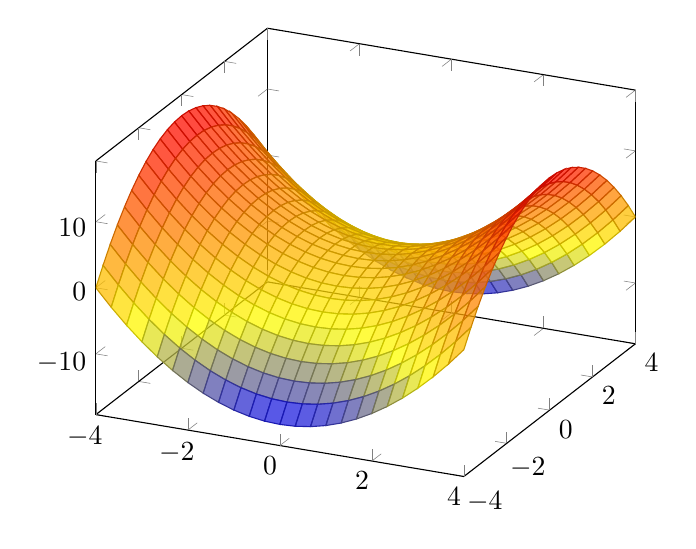
\begin{tikzpicture}
		\begin{axis}[view={25}{30},mark layer=like plot]
			\addplot3 [
				surf,
				shader=faceted,
				fill opacity=0.75,
				samples=25,
				domain=-4:4,
				y domain=-4:4,
				on layer=main,
			] {x^2-y^2};
		\end{axis}
	\end{tikzpicture}
	\caption{An example 3D plot done wit PGFplots.}
\end{figure}

And, of course the code for generating the plot is given as follows:

\begin{code}{latex}
\begin{figure}[!ht]
  \centering
  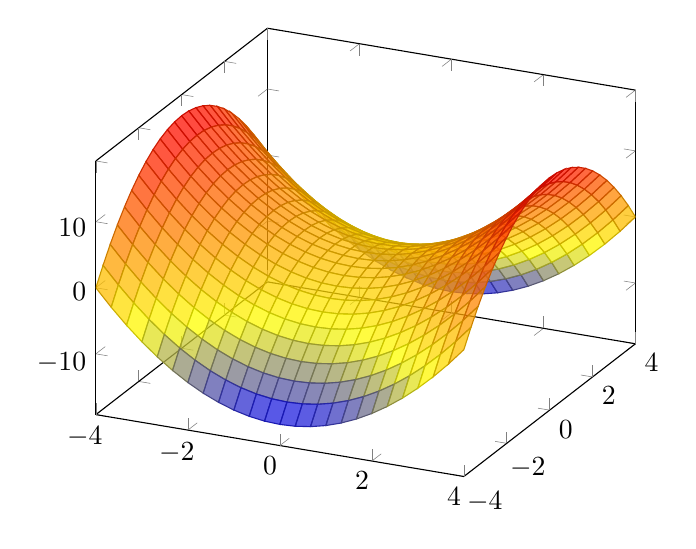
\begin{tikzpicture}
    \begin{axis}[view={25}{30},mark layer=like plot]
      \addplot3 [
      surf,
      shader=faceted,
      fill opacity=0.75,
      samples=25,
      domain=-4:4,
      y domain=-4:4,
      on layer=main,
      ] {x^2-y^2};
    \end{axis}
  \end{tikzpicture}
  \caption{An example 3D plot done wit PGFplots.}
\end{figure}
\end{code}

Some options worth mentioning are as follows:

\begin{hgitemize}
	\item[\pcode{surf}] Generates a \hlight{surface} based on the 2D
	data it was given (in this case these are $x$ and $y$.
	\item[\pcode{shader}] Describes, basically how each segment should be
	filled.
	\item[\pcode{samples}] Similar to 2D plots, tells how many data points will
	be measured. However, make a note that 3D is significantly more taxing
	on the TeX memory than 2D and making this sampling high may result in
	exceeding the memory limit.
\end{hgitemize}

\end{document}

%%% Local Variables:
%%% coding: utf-8
%%% mode: latex
%%% TeX-command-extra-options: "-shell-escape"
%%% TeX-master: t
%%% TeX-engine: luatex
%%% End:

